\chapter{Introduction (outline)}

\section{Amyloid: the field} % (fold)
% Organizational detail: AD and amyloid (which one should go first?). Center it on Amyloid, and then bring in AD as a central motivation for doing amyloid science.

% I think my focus should still be on Alzheimer's disease ... the practical purpose of my work is to understand how inositol works
% I am not trying to cure all amyloid diseases.

\subsection{Alzheimer's Disease}
% Here, my intention is to lead into the discussion of amyloid by giving a historical perspective and overview of AD
% And use AD as a motivation for why so much work has gone into studying amyloids.
\begin{outline}[enumerate]
	\1 More than a hundred years have pass since Dr. Alois Alzheimer first presented the connection between the presence of neuronal plaques and the clinical symptoms of presenile dementia characteristic of Alzheimer's disease (AD).

	\1 Today, AD is known to be the most common cause of dementia in persons of age 65 or older. With the increasing longevity of our population, AD is approaching epidemic proportions with no cures or preventative therapy available.\cite{Blennow:2006wd}

	% Elaborate on happened between the step above and the amyloid hypothesis?
	\1 The discovery of amyloid plaque deposits of the brains of deceased dementia patients led to the formulation of the amyloid hypothesis which posits that amyloid aggregates initiates the pathogenesis of AD, whereas the other numerous symptoms are secondary.

	\1 Decades after the initial discovery by Alois Alzheimer, A$\beta$, the central protein component of neuronal plaques, was synthetically produced in the laboratory. In vitro, A$\beta$ was found to precipitate out of solution almost immediately. 
		\2 Describe the molecular structure of A$\beta$ amyloid fibrils
			\3 Define the cross-$\beta$ structure [Show a schematic here].
		\2 Briefly mention the techniques that can be used to obtain structural information of amyloid fibrils.

% \2 A$\beta$ is produced by intramembrane proteolytic cleavage of the larger amyloid-$\beta$ precursor protein (APP) by $\beta$-secretase, and is produced constitutively as part of the normal cellular metabolism.\{Selkoe, 2002 \#222\} Depending on the position of the cleavage, A$\beta$ peptides of lengths varying from 38 to 43 residues can be produced. However, the peptides spanning residues 1--40 (A$\beta$40) or 1--42 (A$\beta$42) are predominantly found AD-associated plaques.
\end{outline}


\section{Mechanism of amyloid formation and toxicity}
% In this section I will talk about how amyloid aggregation is thought to work. Introduce the thermodynamic model for understanding fibril formation. I will now broadly introduce to amyloid.  
\begin{outline}[enumerate]
	\1 Although the initial studies of amyloid was motivated by attempts to understand the etiology of AD, amyloid science now have grown into its own field.

	\1 Many diseases have been demonstrated to be linked with the presence of amyloid. Type II diabetes, Prion-related diseases, Parkinson's, Huntington's disease etc. Finding a treatment for AD and other fatal neurodegenerative diseases motivated many biochemical and biophysical studies of the amyloid state.  In the laboratory, scientists have been able to produce amyloid from a variety of proteins and peptides, both folded and disordered, via chemical modification of solution conditions and denaturation.

		\2 Amyloid fibrils is formed via a complex aggregation pathway of protein and peptides. Monomers aggregate to form a variety of oligomers with different morphologies, which exists in equilibrium with amyloid fibrils. Some of these oligomers are on-pathway to fibril formation, while others themselves may be end-points of the aggregation pathway. Amyloid fibrils, typically the visible endpoint of aggregation, has a cross-$\beta$ structure.

		\2 Kinetics of amyloid formation.  The formation of amyloid is observed to follow the nucleation-polymerization process. It is characterized by first a slow nucleation-phase, where energetic barriers of aggregation must be overcome to form the initial aggregation nucleus or seed.  Seeding is then followed by a more rapid growth phase (polymerization).

	% Key question in the field: What is the toxic species?
	\1 Toxicity. In recent years, the focus has been on finding the relevant toxic species. The monomeric and fibril forms are thought to be less toxic than oligomers. Multiple lines of research have recently identified oligomers as a likely causative agent for neuronal cell death.  It is hypothesized that oligomers may cause toxicity perturbing the integrity of cellular membranes through binding and disrupting the lipid bilayer (perhaps by making them ion permeable).

		\2 Include a paragraph about amyloid formation and lipid membranes (?)
	% Understanding the toxicity or finding out whether there is a toxic species in part validates the amyloid hypothesis. 

	\1 Because many of insolubility and disordered nature of these oligomeric aggregates, the structure of oligomers have been challenging to obtain via experimental protein structural determination methods.
\end{outline}


\section{Amyloid inhibition by small molecules: a treatment for amyloid disorders}
% Cure, method of prevention; is there hope?
\begin{outline}
	\1 In this section, I will provide an overview of the challenges required to be overcome from a drug perspective to develop a small molecule drug for Alzheimer's disease.  Furthermore, I will motivate why inositol, in particular, is an exciting avenue to explore.
	
	\1 Briefly mention non-small molecule putative therapies which also acts via amyloid inhibition. The focus of this thesis will be on small-molecule amyloid inhibition.
\end{outline}

\subsection{Molecular mechanisms of amyloid inhibition by small molecules}
\begin{outline}[enumerate]
    \1 Amyloid inhibition as a treatment for Alzheimer's disease and related amyloid disorders. Amyloids are attractive drug targets. Small molecules may be one effective way to develop a treatment for amyloid disorders because they have the potential to be able to treat the underlying disease. Through in vitro screening, many small molecules have been found to effect the amyloid aggregation pathway.  Some were demonstrated to inhibit amyloid fibrils, where as others were shown to arrest or reduce oligomer formation.   
      % Here I can take a cue from Justin Lemkul`'s recent review paper.
      % Talk about the different kinds of small molecules that have been found to inhibition amyloid formation.  Here I will also provide a summary of what people know about the mechanism by which they inhibit amyloid formation.
      
      \2 Pharmacological perspective of the challenge of developing an Alzheimer's drug. In order to effectively treat Alzheimer's and other neurodegenerative diseases, small molecule drug candidates must pass the blood brain barrier at sufficient concentrations.  From a pharmacological perspective, this is a difficult to achieve.

      \2 Thioflavin T and Congo red are dye molecules which are used in identifying the presence of amyloid.  Both molecules bind to the fibrillar form of amyloids. They are also both found to inhibit fibril formation.
      
      \2 Polyphenols is a class of molecules which binds to one or species of amyloid. These molecule is found in green tea and wine.  They have anti-oxidative properties.
      
    \1 What do these molecules have in common?
	
		\2 They share common chemical features and groups.  They are typically planar in geometry, have many aromatic rings, and polar functional groups (hydroxyl groups) around the edge of these aromatic rings.
    
    	\2 Mechanism of action. Some small molecules inhibit fibril formation, some inhibits oligomerization. They are all found to be weak binders and act on millimolar concentrations. That is, they are non-specific binders and exert their effects at high concentrations. EGCG, one such polyphenol, is known to have the strongest inhibition properties.
	
	\1 Inositol molecules
	
		\2 The discovery of inositol
		
		\2 Role of inositol in the human body 
		
			\3 \emph{myo}-inositol
			
		\2 Where is inositol found
		
		\2 Role of inositol in amyloid inhibition
		
			\3 in vitro studies
			
			\3 in vivo studies
\end{outline}

\subsection{Analogy to Sugar-protein binding}
% Does this section fit here? Where should I put it?
\subsubsection{Experimental techniques to study sugar-binding modes}
\subsubsection{Sugar Binding modes}


\section{Structure-based Drug Discovery}
\subsection{Forces in protein-ligand interactions}
\begin{outline}
	\1 Interactions important for protein-ligand binding
		\2 Electrostatic interactions: Polar and ionic interactions
			\3 Hydrogen bonding
			\3 Van der Waals / London dispersion forces
		\2 Hydrophobic interactions
\end{outline}

\subsection{Protein-Ligand binding theory}
% subsection protein_ligand_binding_theory (end)
% Below is a summary of an excerpt from Tom's thesis on structure-based drug discovery.
% Design of antibiotics 
% 1) Target determination (biochemical)
% 2) Structural determination (Xray, NMR, or homology); active site identified; Here would be useful to get the holo structure of the protein
% 3) Screen for inhibitors against a chemical library or in silico docking.
\begin{outline}
	\1 Enzyme and the ligand must bind tightly and specifically, so to avoid large drug doses to inhibit the enzyme, which may have adverse side effects (toxicity) in the human body.
	\1 Binding constant is a measure of the affinity of a ligand to a protein. It is the concentration at which 50\% of the drug is bound to the protein. In experimental studies, Kd is often used to identify potential binders. Typically in a classical biochemistry sense/setting, the higher lower the dissociation constant of a drug, the more effective the drug is likely to be.
	\1 Definition of free energies
		\2 Absolute binding free energy
		\2 Relative binding free energy
		\2 Binding equilibrium
			\[ protein+ligand <-> (protein-ligand)aq \]
	\1 Experimental techniques for determining $K_d$. 
		\2 What experimental techniques are used to estimate binding affinity? (Study up on this.)
\end{outline}	

\subsection{Role of chirality in drug binding}
Definition of chirality [Add schematic] ... etc


\section{Molecular Dynamics (MD) Simulations (Beginning of chapter 2?)}
% Motivate MD simulations
\begin{outline}
\1 Molecular dynamics simulations are a useful tool to study the structure, dynamics, and interaction of biomolecules. MD simulations employ an empirical mathematical function to describe the atomic interactions in a molecular system, and together with classical laws of Newtonian mechanics, atomic trajectories of motion are generated. Thermodynamic and kinetic properties can then be extracted as time averages from these trajectories and used to make a number of predictions that are often experimentally challenging to observe or measure.

\1 MD simulation studies have been useful in studying many existing fundamental problems of biology and biochemistry, including protein dynamics and function, protein folding, biomolecular self-aggregation, and protein-ligand binding.
% Study protein dynamics - importance of protein dynamics.
\end{outline}

\subsection{Methodological Details} % (fold)
% Describe the details of molecular dynamics simulations

% A set of numerical computation algorithm which solves numerically solves the N-body problem. Solves a system of Newton's equations of motion, and provides the time-trajectory of atoms with femtosecond time resolution. 

% The integration algorithm is XXX. Time steps used are typically 2 femtoseconds to capture the hydrogen bond vibrational motion. [MORE DETAILS AND EQUATIONS HERE] [Ref: Chris Madill's and Tom's thesis]
% Details of the mathematics (need to review the basic theory + Taylor series expansion) - get a book - tomorrow maybe?

% The assumption at a hand-wave level adapted from Tom's thesis
\begin{outline}
	\1 Why is MD correct? Describe the fundamental assumptions of MD. Here, I want to give the readers who aren't familiar with the methodological details of MD a sense of the rigorousness of MD.
	
		\2 The Born-Oppenheimer approximation: electronic and nuclear motions are uncoupled, and therefore can be treated separately. 
	
		\2 MD does not account for the movement of electrons. Although electrons are not taken into account in MD simulations, their presence is implicitly accounted for via the use of potential energy functions.  Atomic nuclei can be treated as classical particles.

  % \2 Review the basic derivations of MD simulation equations and why they work:
  %   \3 Assume a small integration step (why is 2 fs chosen it is both biological and for numerical stability purposes). Roughly MD follows these steps:
  %     \4 F = -grad E, where E is given by the force field potential energy function.
  %     \4 Determine acceleration for each atom from the forces on each atom
  %     \4 From acceleration determine momentum 
  %     \4 Determine positions

% - Relationship between force and energy 
% - Relationship between momentum and velocity 
% - Why numerical approach must be used (no analytical solution for N > 2)
% - How is the force field plugged into the general algorithm.

  \2 Application of an empirical force field can be used approximate atomic interactions in the system.

      \3 The general force field equation:
      	\[ V(R) = bonds + angles + impropers + dihedrals + pair interactions \]

      \3 There many different force fields (AMBER, Gromos etc), however, in this thesis we apply OPLS-AA force field in all of our simulations.

      \3 The force field has many parameters that need to be determined. One approach is to fit to QM calculations.  Often it is optimal to compute these for small compounds and adjust parameters by comparing calculations to experimental results.

% \1 Steps to produce a molecular simulation:
%   \2 First take a structure from crystallography or NMR, or homology-modelling data.
%   \2 In the algorithm, the forces acting on each atom are estimated from [insert equation here]
\end{outline}

\subsection{Challenges and limitations of MD simulations}
\begin{outline}
	\1 Methodological limitations. MD is computationally challenging because of limitations on length and time scales. 
	
		\2 Length scale. Large systems are too complex to obtain statistics and quantitative predictions.
		
			\3 Convergence
			
		% Evaluating the convergence of simulations is still a challenge
		\2 Time scale. Relevant biochemical reactions such as protein folding happens on the time scale of milliseconds, hours, and days. Currently with MD simulations, we are routinely able to approach the microsecond time scale, massive computing power is still insufficient to observe phenomena on the millisecond timescale. % Ref: DE Shaw Research.
		
	\1 Limitations in the accuracy of current force fields.
\end{outline}		

\subsection{Application of MD to structure-based drug discovery}
\begin{outline}
% \1 (Why computational?) Can help us get protein dynamics is important for understanding protein function. We want to understand protein function because we want to be able to design drugs to cure diseases.

% \1 A important application of MD simulation in biochemistry is the predicting of protein-ligand binding free energies.

	\1 Cheaper, faster, get atomic resolution. Modeling can be used to rapidly prototype an experimental idea -- for example, one can performed computer alchemy, that is, ''mutate``'' residues to test hypothesis. In recent years structure-based computer modeling of protein-ligand interactions have become a core component of modern drug discovery. REF: Mobley, Dill 2004 Computers are advancing thus it is cheaper, MD may be used as a drug discovery platform. In terms of drug discovery, can be used to determine whether a chemical change will produce a more potent drug candidate.

	% MD is more straightforward if there is a folded, protein structure.
	\1 A broad application of simulations of proteins is to computationally design drugs and combining that with structure-based drug design.
	
	  \2 First you solve a protein structure using conventional structural determination methods such as X-ray crystallography or perhaps NMR.  Typically you would have an idea of where the binding pocket is as well. 
	
	  \2 Then taking a protein force field and apply MD simulations to the protein structure in the presence of the putative ligand.  Because the binding affinity is very high (usually the binding specificity ...
	% The sentences above are pretty repetitive. Combine and tighten.

	\1 Typically, an X-ray crystal structure of a target is first determined with a putative binding site. [See Tom's thesis]
	
	\1 Ligands which may act as potential drugs typically have high binding affinity to the binding site. The goal is to find high specificity inhibitor of a protein (usually an enzyme). The binding free energy is an important quantity which can be used to evaluate how well a ligand binds. One method of estimating binding affinity is by using computational docking methods, where the binding affinity is measured without taking into account of the protein conformational entropy.  Although docking is computationally less expensive, it is inaccurate for identifying true drug candidates because binding often involves changes in protein conformation.

	\1 Currently state of the art computational binding studies take into the account of change in protein conformation. MD simulations is an effective method, where the protein and drug is allowed to relax and freely move about in the system.

	\1 However, in the case of very specific binding, observing binding events is a low probability event in MD simulations. Therefore it is not practical to use brute-force MD sampling to determine free energies.

	  \2 Methods used to determine binding free energies using MD:
	  % \3 Linear interaction energy -- Out of scope
	  % \3 MM/PBSA - no explicit account for solvents -- Out of scope
	  	\3 Thermodynamic perturbation \cite{Gilson:2007hz}
			\4 thermodynamic integration
			\4 free energy perturbation
\end{outline}

\section{Amyloid inhibition in the framework of tradition enzyme inhibition mechanism}
\begin{outline}
    \1 Can we think about amyloid inhibition as a standard protein-ligand binding problem? Not really.We have the exact opposite of this framework with amyloids. Most inhibitors are found to be very weak binders ... how are they working as a drug then? And how do we approach this with MD simulations?

    \1 The enzyme and ligand inhibition / binding model cannot be directly applied to understanding amyloid inhibition.  No folded structure, no putative structure (there are many, which one?), no putative binding site (generally presents a surface).

    \1 In AD, there is the added challenge of the drug being able to cross the brain barrier, while remaining non-neurotoxic.  What kind of drugs cross the BBB?  Typically hydrophobic drugs.
\end{outline}    

\section{Review of MD studies of amyloid inhibition by small molecules}
MD studies using brute-force sampling. Aid in medicinal chemistry by making suggestions for how to design new AD drugs

\begin{outline}
	%  Excerpt from Transfer proposal
	\1 In recent years, molecular dynamics simulations have been intensively used to investigate the molecular basis of the structure and stability of amyloid fibrils. However, most of these studies were focused on A$\beta$ and large A$\beta$ aggregates,\{Fawzi, 2008 \#553;Esposito, 2008 \#567;Sgourakis, 2007 \#609;Wei, 2006 \#656;Tarus, 2006 \#628 Karsai, 2006 \#658\} and thus, were computationally limited by the complexity of the molecular systems. To date, few studies have attempted to provide statistically meaningful results pertaining to general mechanisms of protein self-aggregation and amyloid formation. Furthermore, despite the abundance of MD studies of A$\beta$, few studies have systematically examined the mechanism of action of small molecule inhibitors of amyloids. MD simulations of Congo red binding have only been done with the protofibril-like crystal structure composed of the segment GNNQQNY.\{Wu, 2007 \#621\} A recent simulation study of an N-methylated peptide with A$\beta$16-22 models of amyloid aggregates has provided insight into the possible mechanism of action of peptide inhibitors of amyloid formation.\{Soto, 2007 \#597\} This peptide inhibitor was shown to preferentially bind monomers to form dimers, possibly acting to inhibit fibril formation by sequestering monomers. However, peptide-based inhibitors have poor pharmacological profiles as they are actively broken down by proteases in the stomach and are difficult to transport across the blood-brain barrier. In addition, these peptide inhibitors specifically target A$\beta$ and thus do not have the potential to treat multiple amyloid diseases.
\end{outline}

\subsection{Molecular mechanism of binding of dye molecules}
% Review of what is known about dye binding on amyloid fibrils.
Two types of binding modes. Bind flat on amyloid surface. Interact with hydrophobic groups exposed on the amyloid fibrils.
Doesn't explain why the dye molecules are also able to suppress fibril formation.

% Can the birefringence be explained by these binding modes? -- this is out of the scope of my thesis


\section{Thesis objectives and rationale}
\begin{outline}
	\1 Here describe how I designed my study to navigate the challenges presented by the amyloid inhibition problem and MD simulations - rationale. At this point, explain and discuss my approach, study-design and rationale. Include the matrix figure.

	% \begin{figure}
	%   \centering
	%   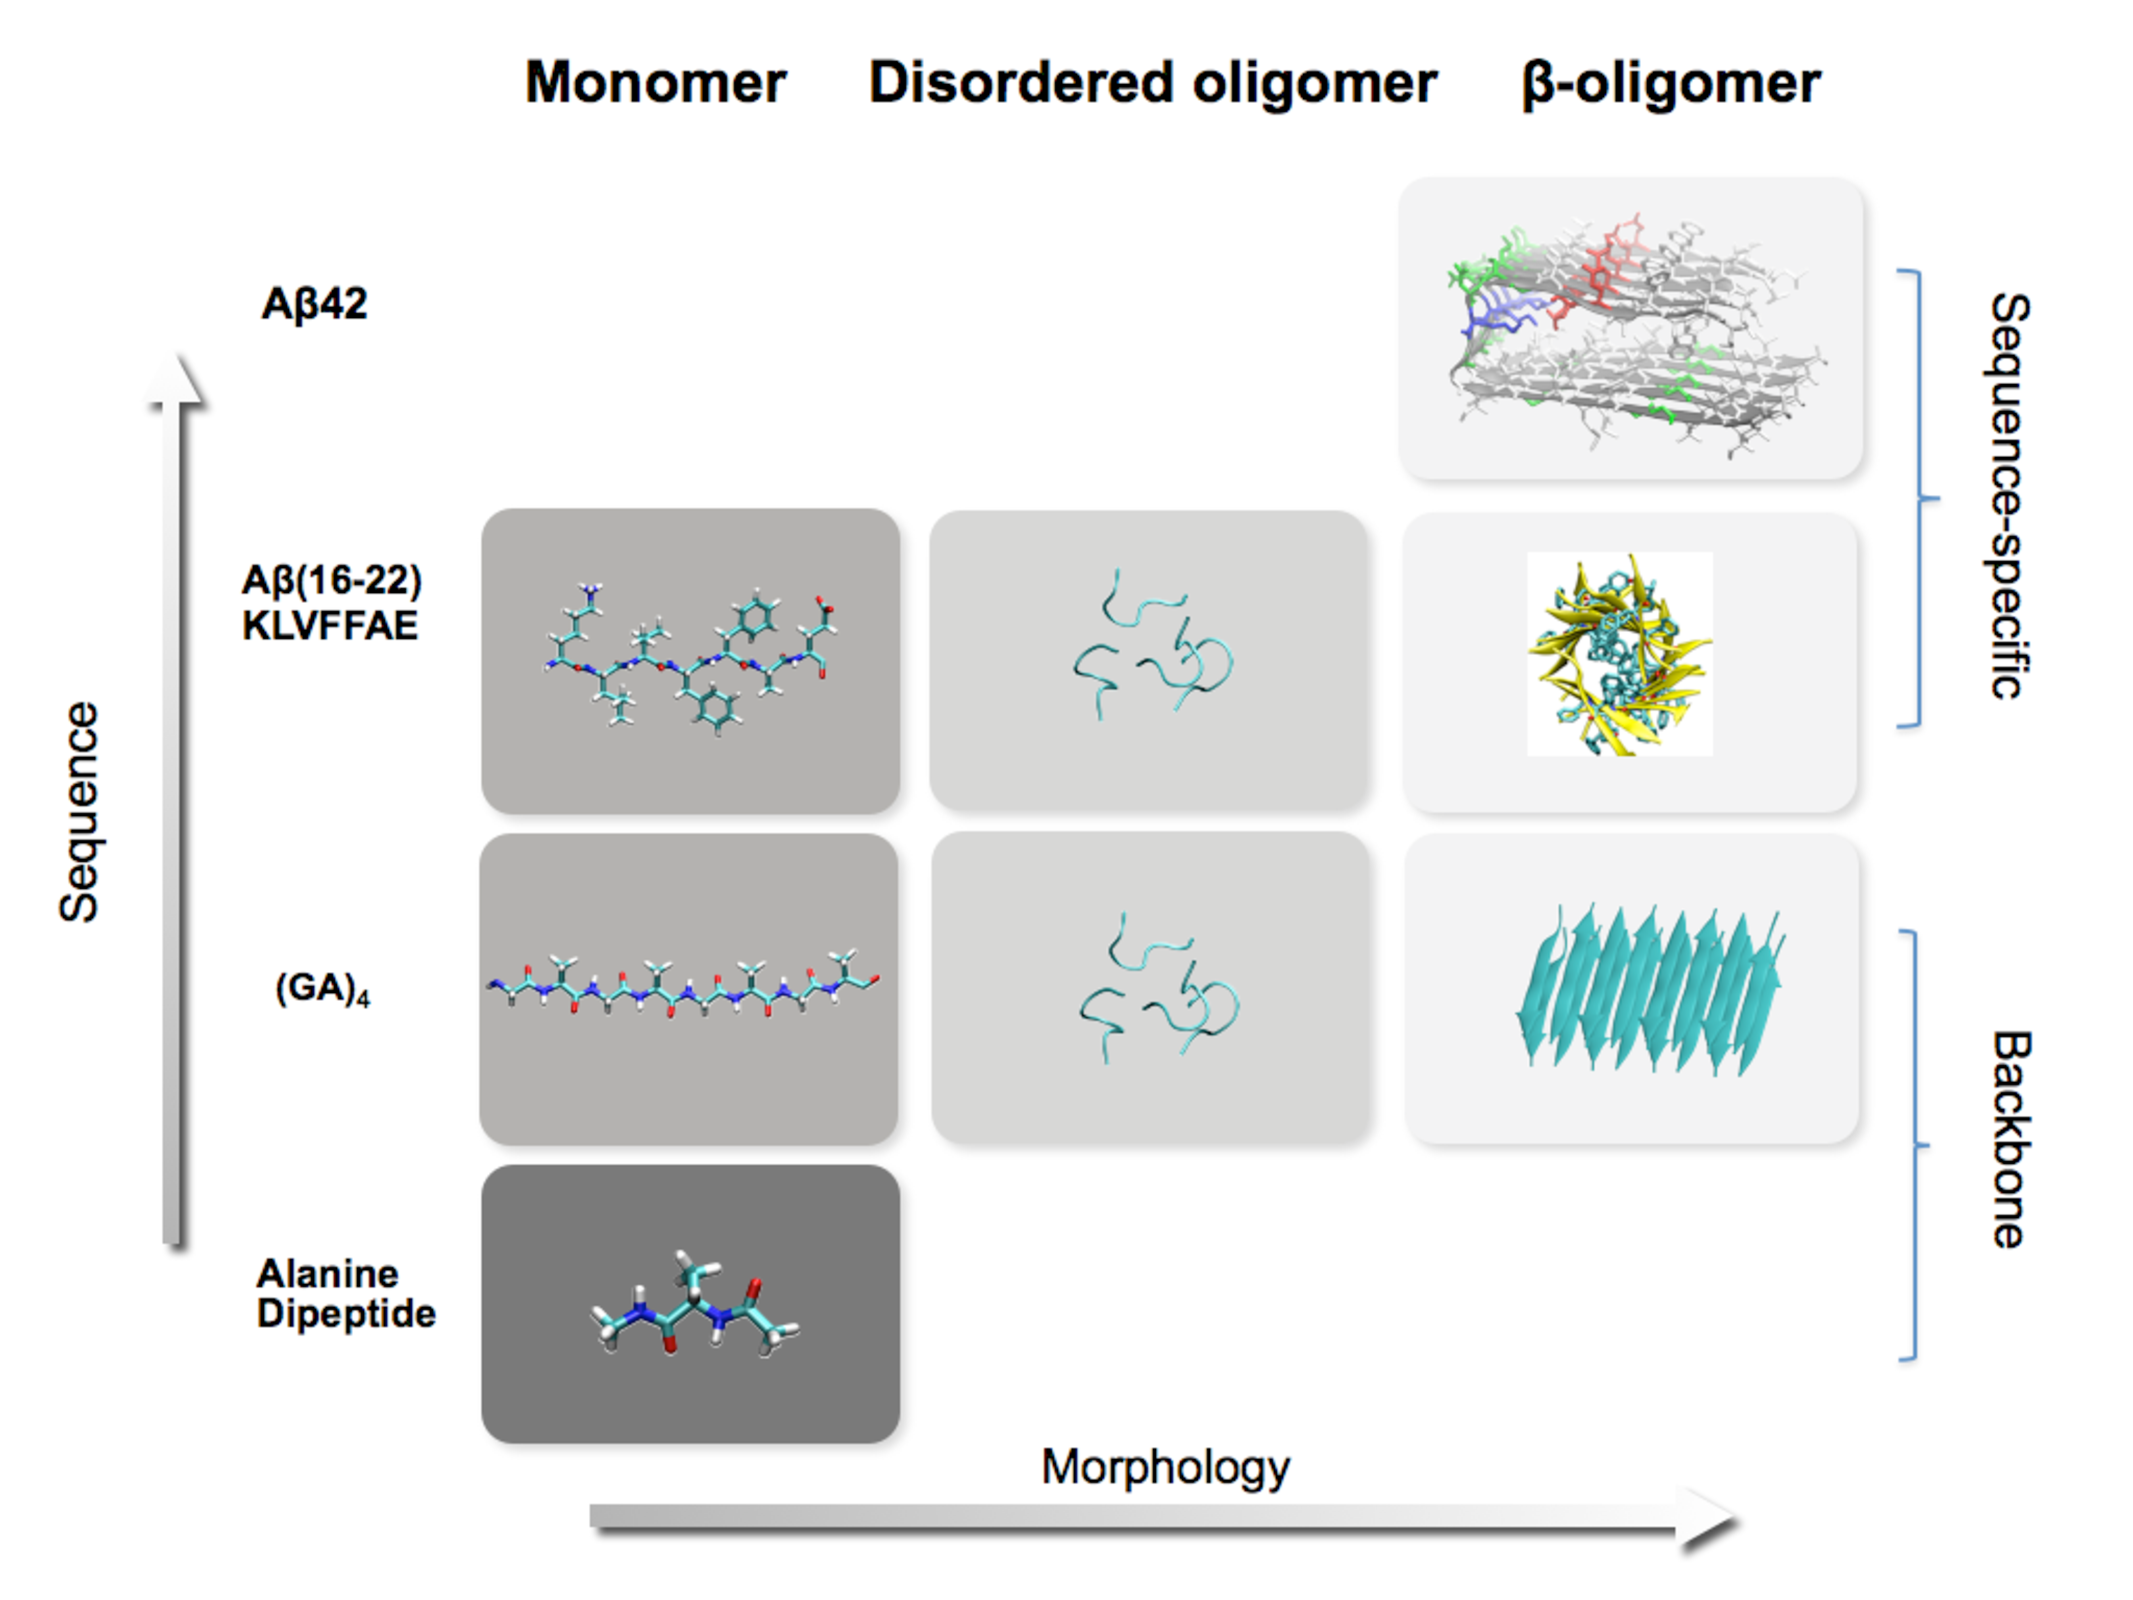
\includegraphics[width=6in]{figures/introduction/matrix.pdf}
	%   \caption[Rationale]{Shows the progression from small, model systems to larger and structurally more complex systems involving the full-length A$\beta$42 peptide.}
	%   \label{fig:rationale}
	% \end{figure}

	\1 A$\beta$ peptides are completely disordered.  Because A$\beta$ amyloid formation consists of many different types of aggregates, a single conformation cannot be assumed for binding.  We also do not know what the binding site looks like, where it is located on these structures.

	\1 Beginning with the simplest model systems for an amyloidogenic peptide, the alanine dipeptide, we systematically examine binding of inositol with systems of both increasing sequence and structural complexity.

	% Use brute force simulations
	\1 We exploit conventional MD simulation techniques because we can't readily pick a reaction coordinate as in tradition enzyme-ligand binding problems. Using large-scale sampling and repeats of many simulations to determine the binding mechanism and binding equilibria.	
\end{outline}

\bibliography{chapter1}